% 1985 广东文史类卷二第四题：直三棱柱题面示意，E 为 AB 中点；不添解答辅助点。
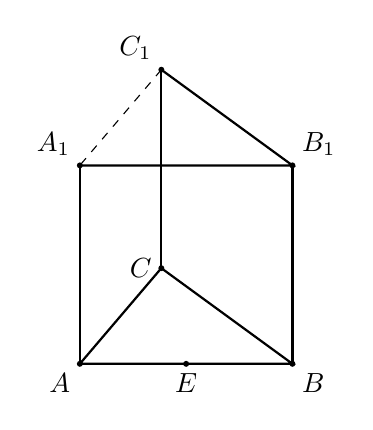
\begin{tikzpicture}[scale=0.9]
  \coordinate (A) at (0,0);
  \coordinate (B) at (3,0);
  \coordinate (C) at (1.15,1.35);
  \coordinate (A1) at (0,2.8);
  \coordinate (B1) at (3,2.8);
  \coordinate (C1) at (1.15,4.15);
  \coordinate (E) at (1.5,0);
  \draw[thick] (A)--(B)--(C)--(A);
  \draw[thick] (A)--(A1) (B)--(B1) (C)--(C1);
  \draw[thick] (A1)--(B1)--(C1);
  \draw[dashed] (C1)--(A1);
  \fill (A) circle (1.2pt) node[below left] {$A$};
  \fill (B) circle (1.2pt) node[below right] {$B$};
  \fill (C) circle (1.2pt) node[left] {$C$};
  \fill (A1) circle (1.2pt) node[above left] {$A_1$};
  \fill (B1) circle (1.2pt) node[above right] {$B_1$};
  \fill (C1) circle (1.2pt) node[above left] {$C_1$};
  \fill (E) circle (1.2pt) node[below] {$E$};
\end{tikzpicture}
